\documentclass[preprint,12pt]{elsarticle}
\usepackage[T1]{fontenc}
\usepackage[utf8]{inputenc}
\usepackage{lmodern}
\usepackage{booktabs,tabularx,array,longtable}
\usepackage{microtype}
\usepackage{graphicx}
\usepackage{url}
\usepackage[hidelinks]{hyperref}
\emergencystretch=3em
\title{Supplementary Material: A Multi-Axis Empirical Audit of Machine-Learning Intrusion Detection}
\author[anon]{AUTHOR\_CONFIRMATION\_REQUIRED}
\address[anon]{AUTHOR\_CONFIRMATION\_REQUIRED}
\begin{document}
\maketitle
\section*{Use and evidence boundary}
This supplement contains reviewer-facing frozen evidence and provenance records. It does not redistribute restricted datasets, raw traffic, private information, closed scientific targets, unauthorized model checkpoints, or the complete research repository. Values retain their source populations, native metrics, uncertainty semantics, and qualifications. Static verification is not represented as a complete end-to-end experimental rerun. Source paths and SHA-256 values are recorded in \texttt{source-manifest.csv}.

\section{S1. Reference evaluation, uncertainty, and explanation reliability}
The processed CSE-CIC-IDS2018 reference is a rebalanced within-table condition. Its six frozen membership counts, threshold roles, operating metrics, calibration records, paired conditional intervals, seed summaries, LIME reliability diagnostics, and TreeSHAP comparisons remain governed by the revision manuscript and Stage 29 registries. No learner-winner claim is introduced. The complete approved reference source is recorded in \texttt{source/RESULTS\_SUMMARY.md}; unavailable historical arrays and closed targets remain unavailable.

\subsection*{S1 evidence record}
Population: processed, rebalanced CSE-CIC-IDS2018 holdout. Metrics: F1, F2, FPR, ROC-AUC, PR-AUC, Brier score, and declared conditional intervals. Qualification: reference evidence does not establish natural prevalence, temporal validity, transfer, or deployment utility. The source manifest records the copied authority and hash.

\section{S2. Shortcut, representation, and architecture diagnostics}
The approved Stage 23 table records the primary frozen subset intervention. It is presented as feature-set sensitivity, not proof of leakage or causality. Matched-size placebos, depth-one controls, attribution proxies, behavior-restricted representations, and family-composition evidence retain their original status. Stage 18 graph and Stage 21 CNN/ViT materials remain supplement-only and descriptive; no architecture or deployment superiority claim is promoted.

\subsection*{S2 evidence record}
The copied table \texttt{source/table\_23\_1\_primary\_subset\_performance.csv} is the approved primary subset artifact. Population: frozen random-natural and chronological-natural populations. Metrics: native ranking and operating metrics as recorded. The remaining Stage 23 and Stage 21 artifacts are repository dependencies, not silently reconstructed here.

\section{S3. Cross-dataset contracts and sensitivity}
Bridge62 and bridge70 are direction-specific semantic contracts. IDS2018-to-CICIDS2017 and CICIDS2017-to-IDS2018 remain separate; they are not averaged. Published-versus-corrected aggregate-flag effects retain metric-specific changes. The two planned \texttt{GROUNDED\_S4} cells remain cancelled because exact durable physical-row membership was unavailable before target opening.

\subsection*{S3 Table S1. Directional transfer source}
The following exhibit is copied from the approved publication table; no values were recomputed.
\begin{table}[htbp]
\centering\small
\caption{Approved bidirectional bridge62 source artifact.}
\begin{tabularx}{\textwidth}{@{}lX@{}}
\toprule
Field & Value\\
\midrule
Source artifact & \texttt{source/table24\_1\_bidirectional\_generalization.csv}\\
Population & Separate frozen source-to-target bridge62 directions\\
Metrics & PR-AUC, ROC-AUC, target prevalence\\
Qualification & Directions use different learners, populations, and target roles; no pooled score\\
\bottomrule
\end{tabularx}
\end{table}

\section{S4. Prevalence, workload, capacity, and cost}
The approved operational translation is an analytic prior-shift projection. Sensitivity and false-positive rate are held fixed while prevalence varies. Traffic volume, analyst service time, capacity, and relative costs are scenarios, not field measurements. The copied source table records the selected 0.1\% operating-point translations. Full grids, break-even conditions, and cost decisions remain identified in the source registry; no new formula or value is introduced here.

\section{S5. Deployment profiling}
Deployment profiling is bounded from prepared model input to materialized probabilities on the recorded hardware and software. Warm/cold inference, throughput, memory, package size, component timings, batch schedules, representation groups, and backend statuses retain separate populations. Unsupported, incompatible, timed-out, and resource-limited paths remain statuses rather than imputed measurements. Capture, flow extraction, external representation construction, alert aggregation, and analyst response are outside the measured boundary.

\subsection*{S5 evidence record}
Copied source artifacts include CPU warm inference and the approved Stage 26 publication tables. Population: compatible paths at the recorded hardware/software boundary. Metrics: latency, throughput, memory, package size, and status fields as declared by each table. No timing was regenerated.

\section{S6. LOAO eligibility and realization stability}
LOAO requires zero training and validation exposure to the eligible target family, day-atomic ordering, and sufficient support. DDoS, Port Scan, Web Attack, Bot, and Infiltration remain separate. Infiltration is descriptive at support 36. DOS and AUTH\_BRUTE\_FORCE remain structurally ineligible. No pooled novelty score is formed.

\begin{figure}[htbp]
\centering
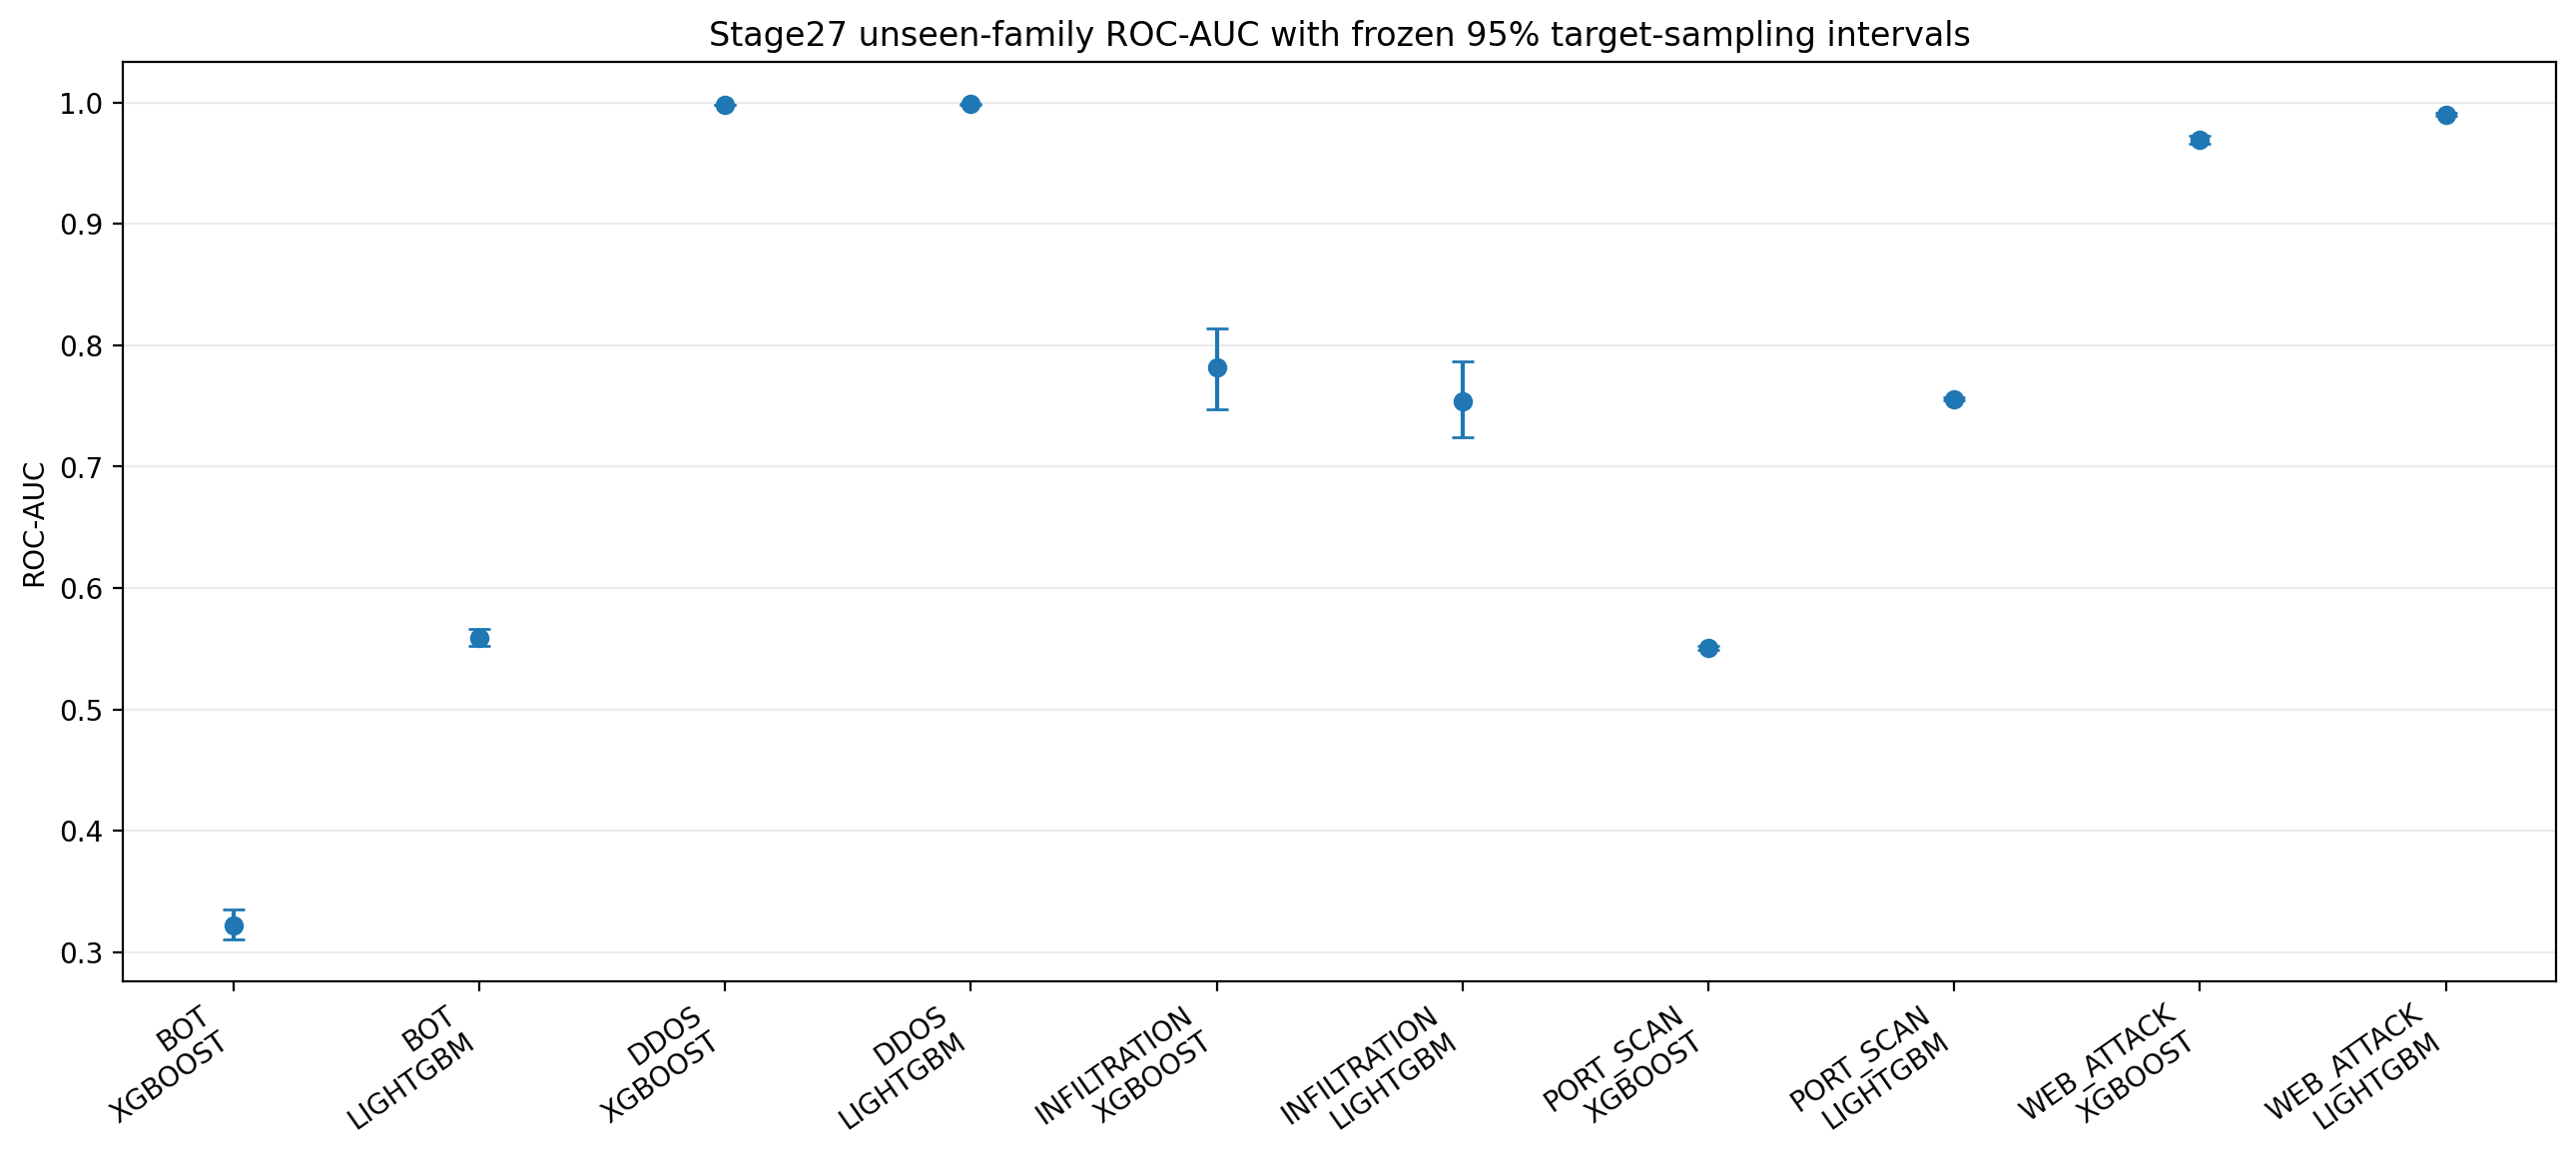
\includegraphics[width=0.95\textwidth]{figures/stage27_primary_roc_auc_ci.png}
\caption{Figure S1. Approved LOAO ROC-AUC evidence. Frozen family-specific conditional intervals remain conditional; this exhibit does not represent an aggregate future-attack score.}
\end{figure}
\begin{figure}[htbp]
\centering
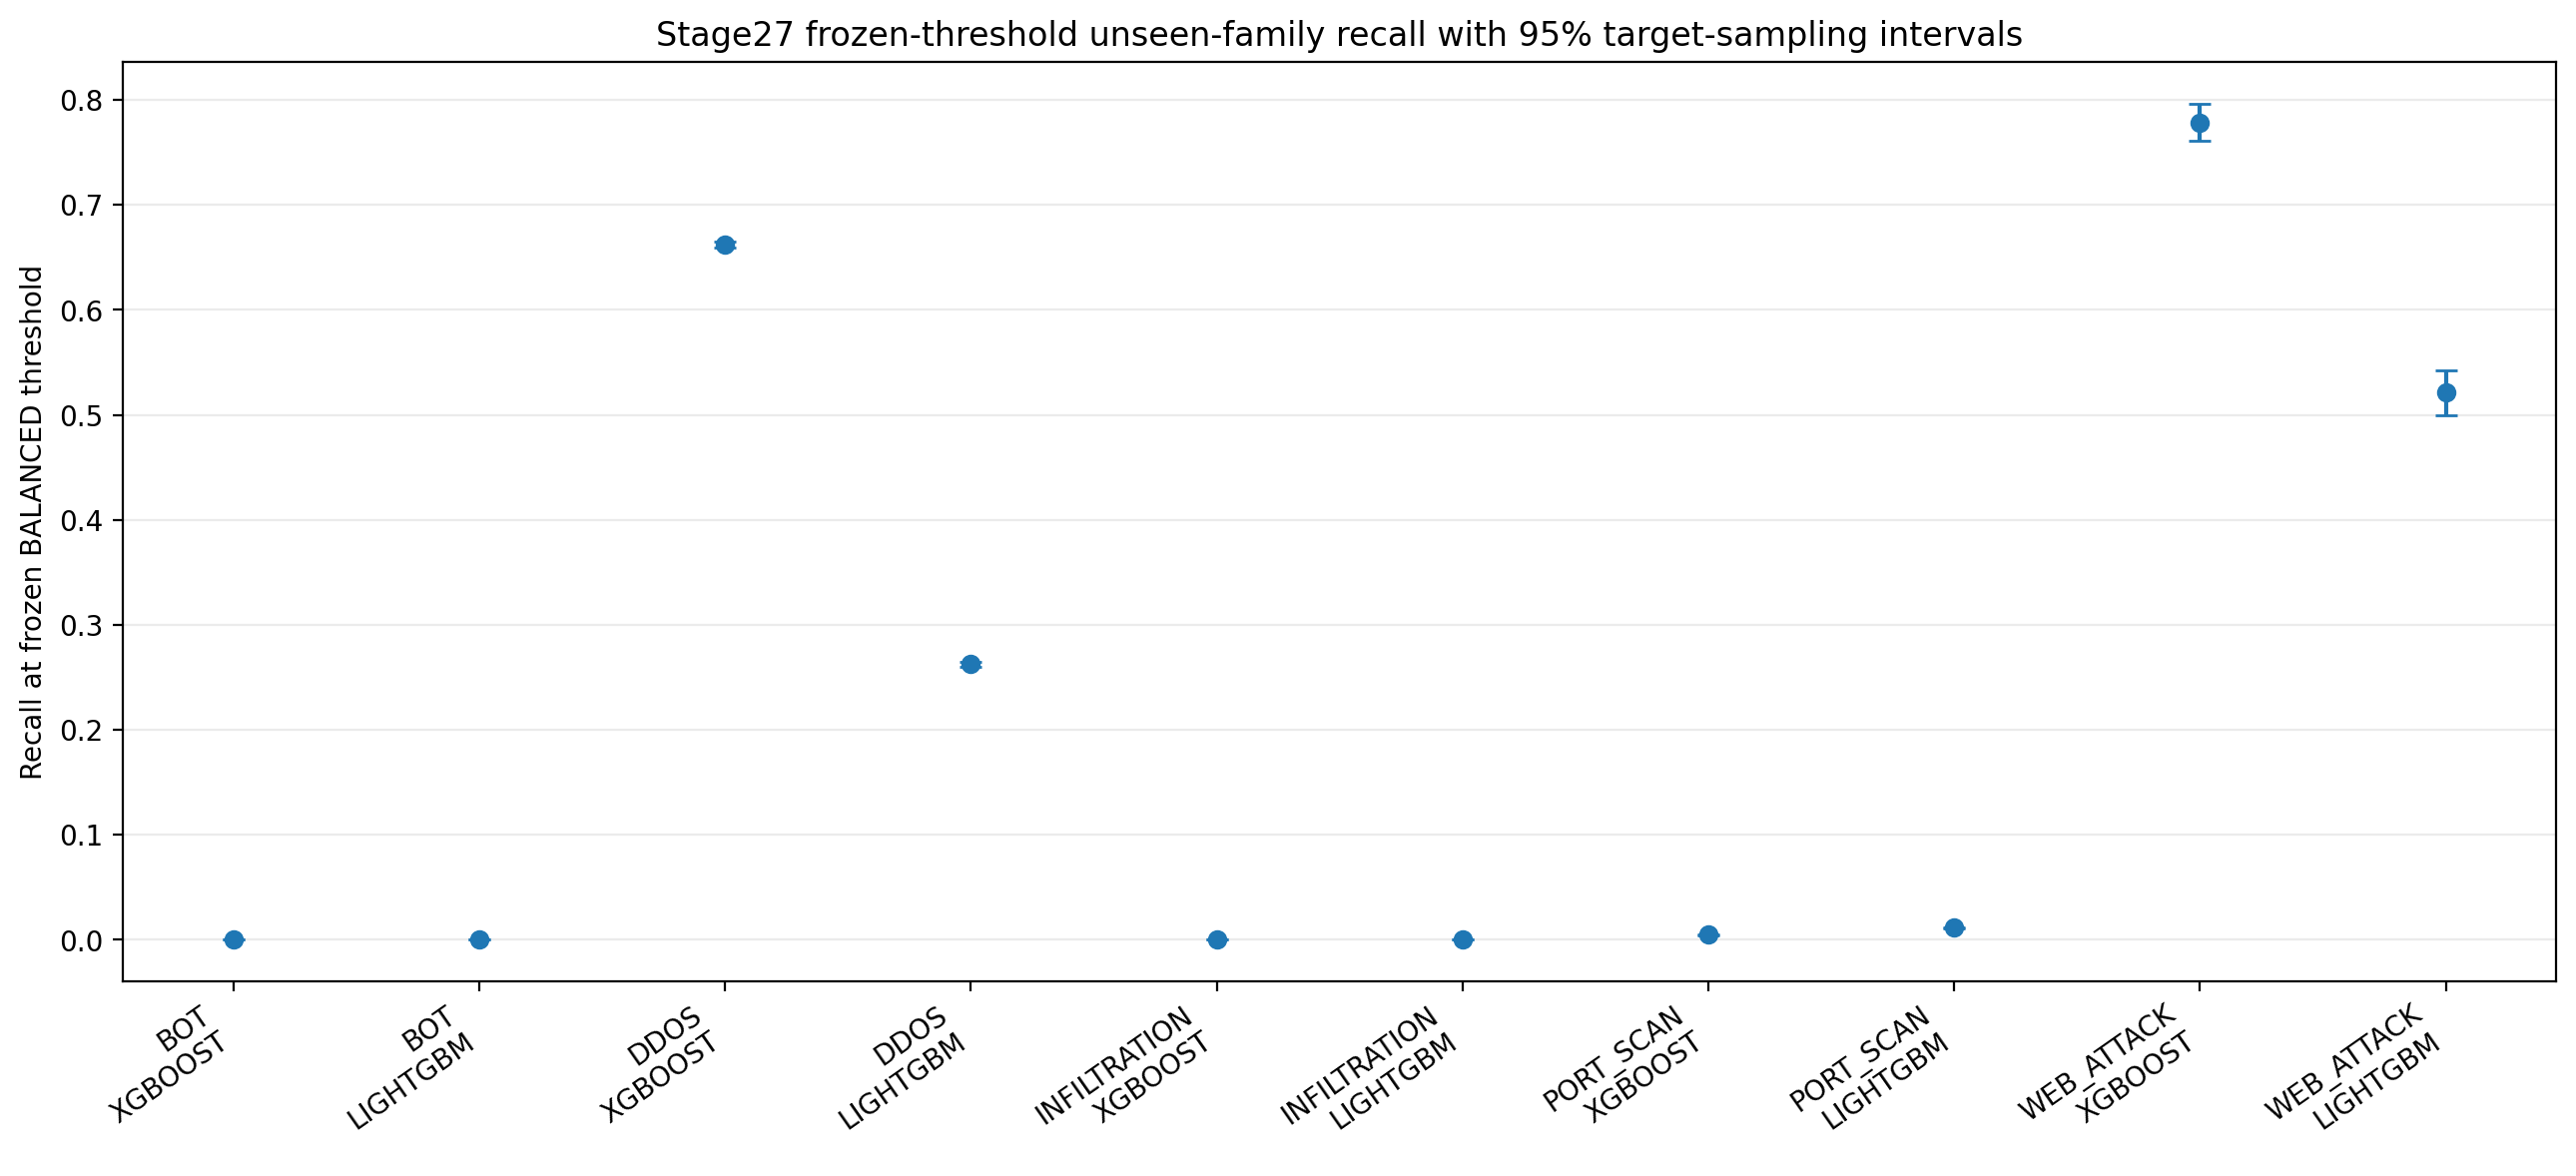
\includegraphics[width=0.95\textwidth]{figures/stage27_balanced_recall_ci.png}
\caption{Figure S2. Approved LOAO balanced-threshold recall evidence. Family eligibility, support, learner, and threshold qualifications remain attached.}
\end{figure}

The copied Stage 28 seed summary and LOAO stability registry preserve the five-seed temporal ordering, registered realization rules, learner dependence, support limits, and historically opened target boundary. No best seed was selected.

\section{S7. Provenance, equivalence, and reproduction}
The package records source paths and hashes for every copied exhibit in \texttt{source-manifest.csv}. The authoritative project retains claim-to-artifact mappings, configurations, source maps, environment records, target-opening ledgers, equivalence matrices, reproduction indexes, and static validation reports. Some environments remain \texttt{VERSION\_NOT\_PROVEN}; some raw data, historical environments, models, arrays, and closed targets are unavailable. The repository therefore supports claim-level traceability, not complete local regeneration of every result.

\subsection*{Redistribution and dependency record}
Only approved editorial tables, documentation, and registered public figure assets are copied here. Restricted original datasets, raw packet records, private information, unauthorized checkpoints, and closed targets are excluded. Any exhibit not copied because its source or redistribution status could not be verified remains a documented dependency rather than a fabricated placeholder.

\section*{Supplement production QA}
Seven sections are populated with frozen evidence descriptions. Tables S1 and Figures S1--S2 are explicitly identified. Every copied source is listed with hash, population, metrics, and qualification in the source manifest. No scientific computation occurred during assembly. The main manuscript references this separate supplement; final author and venue review remain required.
\end{document}
